\documentclass[sn-mathphys]{sn-jnl}% Math and Physical Sciences Reference Style
%%\documentclass[sn-aps]{sn-jnl}% American Physical Society (APS) Reference Style
%%\documentclass[sn-vancouver]{sn-jnl}% Vancouver Reference Style
%%\documentclass[sn-apa]{sn-jnl}% APA Reference Style
%%\documentclass[sn-chicago]{sn-jnl}% Chicago-based Humanities Reference Style
%%\documentclass[sn-standardnature]{sn-jnl}% Standard Nature Portfolio Reference Style
%%\documentclass[default]{sn-jnl}% Default
%%\documentclass[default,iicol]{sn-jnl}% Default with double column layout

\usepackage{graphicx} 
\usepackage{subfig}

%%%% Standard Packages
%%<additional latex packages if required can be included here>
%%%%

\jyear{2023}%

%% as per the requirement new theorem styles can be included as shown below
\theoremstyle{thmstyleone}%
\newtheorem{theorem}{Theorem}%  meant for continuous numbers
%%\newtheorem{theorem}{Theorem}[section]% meant for sectionwise numbers
%% optional argument [theorem] produces theorem numbering sequence instead of independent numbers for Proposition
\newtheorem{proposition}[theorem]{Proposition}% 
%%\newtheorem{proposition}{Proposition}% to get separate numbers for theorem and proposition etc.

\theoremstyle{thmstyletwo}%
\newtheorem{example}{Example}%
\newtheorem{remark}{Remark}%

\theoremstyle{thmstylethree}%
\newtheorem{definition}{Definition}%

\raggedbottom
%%\unnumbered% uncomment this for unnumbered level heads

\begin{document}

\title[Article Title]{Reinforcement-Tracking: an end-to-end trajectory tracking method based on self-attention mechanism}


%%=============================================================%%
%% Prefix	-> \pfx{Dr}
%% GivenName	-> \fnm{Joergen W.}
%% Particle	-> \spfx{van der} -> surname prefix
%% FamilyName	-> \sur{Ploeg}
%% Suffix	-> \sfx{IV}
%% NatureName	-> \tanm{Poet Laureate} -> Title after name
%% Degrees	-> \dgr{MSc, PhD}
%% \author*[1,2]{\pfx{Dr} \fnm{Joergen W.} \spfx{van der} \sur{Ploeg} \sfx{IV} \tanm{Poet Laureate} 
%%                 \dgr{MSc, PhD}}\email{iauthor@gmail.com}
%%=============================================================%%

\author[1,2]{\fnm{Weiming} \sur{Liao}}\email{mingx@stumail.ysu.edu.cn}

\author*[2,3]{\fnm{Guanglei} \sur{Zhao}}\email{zglmj@ysu.edu.cn}
\equalcont{These authors contributed equally to this work.}

\author[1,2]{\fnm{Zihao} \sur{Chen}}\email{476379292@qq.com}
\equalcont{These authors contributed equally to this work.}

\affil*[1]{\orgdiv{The Insititute of Electrical Engineering}, \orgname{Yanshan University}, \orgaddress{\street{Hebei Street West}, \city{Qinhuangdao}, \postcode{066004}, \state{ Hebei}, \country{China}}}

%%==================================%%
%% sample for unstructured abstract %%
%%==================================%%

\abstract{As a bridge between planners and actuators, trajectory tracking is a critical and essential part of robot navigation, autonomous driving and other fields. While traditional trajectory tracking methods generally have disadvantages such as poor tracking accuracy, high modeling requirements, and heavy computational load.This paper proposes an end-to-end trajectory tracking method based on reinforcement learning, and an information encoding network and a reinforcement learning policy network are constructed. A multi-task dense reward function for trajectory tracking is designed.For efficient encoding of local trajectory information, a self-attention mechanism is introduced.A virtual simulation environment is constructed for model training by modeling the trajectory tracking task.Comparing the proposed method with model predictive control and pure pursuit in the tracking experiments of several reference trajectories. The results show that our proposed method has significant advantages in terms of lateral tracking.}

%%================================%%
%% Sample for structured abstract %%
%%================================%%

% \abstract{\textbf{Purpose:} The abstract serves both as a general introduction to the topic and as a brief, non-technical summary of the main results and their implications. The abstract must not include subheadings (unless expressly permitted in the journal's Instructions to Authors), equations or citations. As a guide the abstract should not exceed 200 words. Most journals do not set a hard limit however authors are advised to check the author instructions for the journal they are submitting to.
% 
% \textbf{Methods:} The abstract serves both as a general introduction to the topic and as a brief, non-technical summary of the main results and their implications. The abstract must not include subheadings (unless expressly permitted in the journal's Instructions to Authors), equations or citations. As a guide the abstract should not exceed 200 words. Most journals do not set a hard limit however authors are advised to check the author instructions for the journal they are submitting to.
% 
% \textbf{Results:} The abstract serves both as a general introduction to the topic and as a brief, non-technical summary of the main results and their implications. The abstract must not include subheadings (unless expressly permitted in the journal's Instructions to Authors), equations or citations. As a guide the abstract should not exceed 200 words. Most journals do not set a hard limit however authors are advised to check the author instructions for the journal they are submitting to.
% 
% \textbf{Conclusion:} The abstract serves both as a general introduction to the topic and as a brief, non-technical summary of the main results and their implications. The abstract must not include subheadings (unless expressly permitted in the journal's Instructions to Authors), equations or citations. As a guide the abstract should not exceed 200 words. Most journals do not set a hard limit however authors are advised to check the author instructions for the journal they are submitting to.}

\keywords{Reinforcement learning, trajecotry tracking, self-attention}

%%\pacs[JEL Classification]{D8, H51}

%%\pacs[MSC Classification]{35A01, 65L10, 65L12, 65L20, 65L70}

\maketitle


%\begin{CJK*}{UTF8}{gbsn}


\section{Introduction}\label{sec1}

The autonomous movement and navigation capabilities of unmanned ground vehicles (UGVs) have greatly improved due to rapid advancements in computer technology and artificial intelligence in recent years. And among the most popular and reliable approaches to achieving autonomous navigation is the perception-planning-control navigation pipeline\cite{b.ravikiranDeepReinforcementLearning2021}. This pipeline has been widely adopted in various autonomous systems, such as service robots, self-driving cars, and unmanned aerial vehicles, to accomplish navigation tasks. The trajectory tracking control, serving as an intermediate bridge between the planning and execution layers within this approach, plays a pivotal role in determining the effectiveness and overall performance of the autonomous navigation system.


In practical trajectory tracking control, several factors can affect the performance of path tracking, including the nonholonomic constraints of the unmanned vehicle. The constraints of the kinematic and dynamic models can impact the trajectory tracking performance in real control situations. Additionally, the actuator performance constraints, such as the unmanned vehicle's speed and minimum turning radius can limit system performance. Different control strategies are necessary to meet these intrinsic requirements to accommodate various constraints. Situational constraints also play a critical role in trajectory tracking. For instance, in autonomous driving situations, passenger comfort and lane centerline maintenance are important considerations.

To summarize, different trajectory-tracking control methods are necessary to accommodate distinct control requirements. Preview-based tracking control approaches can produce effective results for trajectory tracking with moderate speed and less extreme curvature changes. In contrast, optimization-based trajectory tracking methods can handle high dynamic scenarios but may have drawbacks, such as design complexity and relatively long response time, which limit their widespread use. Moreover, the performance of the controller depends on the accuracy of the model.

Reinforcement learning (RL) has made significant advances in recent years due to the progress made in deep learning and hardware technology. This progress has led to the increasing utilization of RL in academic settings to address control and decision-making issues\cite{chenInterpretableEndtoEndUrban2022,huangEndtoEndAutonomousDriving2019}. The utilization of RL has simplified controller design and provided superior control outcomes with sufficient appropriate samples. Moreover, it enables the implementation of sophisticated and highly dynamic trajectory tracking control, such as turning operations on roads\cite{hilleliDeepReinforcementLearning2018}.

In light of the aforementioned challenges, this paper presents a new end-to-end trajectory tracking method based on Dueling Double Deep Q-networks(DDQN)to achieve effective control of complex motion trajectories. Rather than using global reference trajectory information, our approach employs local reference trajectory as input for trajectory tracking. When processing reference trajectory data, a self-attention mechanism is introduced to extract useful information from trajectory segments, resulting in a smaller model and a quicker response speed. Regarding the reward strategy, we employ a dense rewards policy to enable efficient network training. Moreover, we introduce a Lattice Graph method in the action space extraction to achieve better discrete control and reduce the training time\cite{pivtoraikoDifferentiallyConstrainedMobile2009}. 


Through experimental comparison, our designed controller has higher control frequency compared to the optimization-based controller. Meanwhile, our controller delivers better control performance than the preview-based approach.

\section{Related works}\label{sec2}
\textbf{Preview-Based trajectory tracking controllers}


The common feature of the preview-based control methods is that a point on the reference trajectory is selected as the preview point, and the control output is calculated based on the relative relationship between the preview point and the unmanned vehicle.The most widely-used and straightforward method for trajectory tracking is the Proportional-Integral-Derivative (PID) based tracking control method, which often involves decoupling the control of the unmanned vehicle into horizontal and vertical components to achieve effective trajectory tracking. Fractional Order PID (FOPID) is utilized for path tracking control and effectively reduces the overshoot of the system, despite the unmanned vehicle trajectory tracking control having a high degree of nonlinear and dynamic features.\cite{ammarRobustPathTracking2020}.
In order to overcome the shortcomings of the lack of a system model for PID, geometric model-based lateral tracking methods have been proposed. Common methods include pure pursuit control, which calculates the vehicle control angle based on the geometric relationship, essentially converting the lateral error between the vehicle location and the desired trajectory at the pre-sighting point into a controlled quantity, thus reducing the deviation\cite{samuelReviewPurepursuitBased2016}.
Stanley's method takes the front wheel of the unmanned vehicle as the center and takes into account the lateral error and the deviation of heading angle, and realizes path tracking by the control of the front wheel turning angle.\cite{sniderAutomaticSteeringMethods2009}.
The benefit of the above control methods is that complex models are not required. 
While these methods fail to take into account the dynamics of the vehicle, as a result, the steady-state error of the control system will increase as the speed increases, which makes it difficult to cope with high-speed motion scenarios.

\textbf{Optimization-Based trajectory tracking controllers}

Aiming at the issues of preview-based approaches, the linear quadratic regulator(LQR) tracking control based on the optimal control theory is developed, and the lateral controller is designed by establishing the vehicle dynamics model, which greatly improves the tracking performance. However, the control of real vehicles often has various constraints, and the LQR control is difficult to handle the constraints flexibly. Meanwhile, the algorithm is for whole time domain control, and the anti-interference ability is not strong. When the curvature varies quickly, there is a significant overshoot, which can easily lead to system instability\cite{amerModellingControlStrategies2017}.
In order to overcome this series of issues, Trajectory tracking control based on model predictive control(MPC) has been proposed. MPC uses the predictive model of the system to predict the future state and determines the control sequence by the receding optimization while taking into account various constraints. Feedback correction is used to continuously adjust the control output at the sampling moment to achieve finite time-domain control of the system.\cite{7320765}.
Whereas it also creates new problems because receding optimization increases the algorithm's time complexity, places heavy demands on the hardware, and causes the calculation time to grow exponentially with model complexity. In the article \cite{chenMPCbasedPathTracking2020a}, The authors embed the PID speed controller into the model predictive control controller to reduce the computational effort of solving the optimization problem and achieve the tracking of the continuous and fast-changing trajectory of curvature. However, MPC is a model-based control algorithm, and the model limits the control performance. In complex scenarios, how to construct an accurate model directly affects its control performance, which greatly limits the design and generality of the controller.

\textbf{Deep learning methods}

In order to reduce the complexity of the controller, many researchers want to implement end-to-end navigation systems by using sensors as input and neural networks to learn navigation or path tracking. It can achieve optimal performance with sufficient training samples\cite{bojarskiEndEndLearning2016}.
In study \cite{mullerOffroadObstacleAvoidance2005}, the authors utilized image inputs from dual cameras and a 6-layer convolutional neural network to establish the mapping between the images and the turning angle of the car to achieve end-to-end lateral trajectory tracking control. 
Despite the effectiveness of deep learning techniques, they are constrained by their limited generalization capability, which limits their applicability in real-world systems. In order to enhance the performance of control systems, several researchers have merged neural networks with conventional feedback feedforward controllers. For instance, Spielberg et al. \cite{spielbergNeuralNetworkVehicle2019} utilized neural networks and feedback control to design controllers and evaluate their performance in vehicle control. The study's findings revealed that this integrated approach outperforms the control of professional drivers, demonstrating that combining deep learning methods with conventional control methods could be an effective strategy to enhance the performance and stability of control systems.

\textbf{Reinforce learning methods}

Reinforcement learning is an emerging approach to solving robot control challenges \cite{zhaoPathFollowingOptimization2021a}, which learns optimal control strategies to maximize periodic cumulative rewards through the interaction of intelligence with its environment. Deep reinforcement learning employs neural networks to approximate state value functions or policies, enabling it to adapt to complex environmental changes and effectively handle nonlinear and high-dimensional control problems. As a result, this approach has been widely used in the field of complex robot control\cite{koberReinforcementLearningRobotics2013, dasilvaSurveyTransferLearning2019}. In the task of trajectory tracking control, the authors propose trajectory tracking control methods based on Deep Deterministic Policy Gradient(DDPG) \cite{lillicrapContinuousControlDeep2019}, which incorporates Actor-critic algorithms \cite{kondaActorcriticAlgorithms1999}, deterministic policy gradient \cite{silver2014deterministic}, DQN algorithm \cite{mnihPlayingAtariDeep2013a} to implement the path tracking control of vehicles in TORCS simulation. Nevertheless, the DDPG algorithm may encounter issues such as overestimation of state action values, large cumulative errors, and low training efficiency \cite{fujimoto2018addressing}. To tackle these challenges, certain researchers have integrated a dual evaluation network and prioritized experience replay mechanism to enhance the performance of the DDPG algorithm and facilitate its application in the lane holding task of autonomous vehicles\cite{heLaneFollowingMethod2021}. Liu et al. use point cloud data and satellite maps to extract real reference road information and generate reference trajectories. They further enhanced the trajectory tracking performance by integrating imitation learning and reinforcement learning, which resulted in accurate trajectory tracking control for urban roads\cite{liuReinforcementTrackingEffectiveTrajectory2022}. Nevertheless, while reinforcement learning algorithms tend to perform well in simulations, deploying them in real-world applications often requires substantial effort \cite{guDeepReinforcementLearning2017}.






\section{Trajectory tracking process and environment}\label{sec3}
\subsection{Markov decision process(MDP)}\label{subsec1}
The Markov Decision Process (MDP) serves as the fundamental framework for reinforcement learning, enabling the representation of agent-environment interactions. MDP embodies the Markov property, which stipulates that the conditional probability distribution of a random process's future state, given the current state and all previous conditions, is solely determined by the present state. Consequently, the actions of an agent in the current state exert an influence on both present and future returns\cite{8585411}. Let the sequence of random variables with Markov property be $s_1,s_2,\cdots,s_t$,which satisfies:

\begin{equation}
p\left(s_{t+1} \mid s_{t}\right) =p\left(s_{t+1} \mid s_1,s_2,\cdots,s_t\right)
\end{equation}

In the Markov process, the introduction of a reward function results in the formation of a Markov reward process (MRP).In order to distinguish the importance of the reward, the discount factor $\gamma$is introduced, and the cumulative discount return after time $ t $ is as follows:
\begin{equation}
G_{t}=r_{t+1}+\gamma r_{t+2}+\gamma^{2} r_{t+3}+\gamma^{3} r_{t+4}+\ldots+\gamma^{T-t-1} r_{T}
\end{equation}
Where,$T$is the final moment, and $r(t)$is the reward at the moment t

The state value function V(s) in the process of MRP is calculated by expectation and expressed as:
\begin{equation}
\begin{aligned}
V(s) &=\mathbb{E}\left[G_{t} \mid s_{t}=s\right] \\
&=\mathbb{E}\left[r_{t+1}+\gamma r_{t+2}+\gamma^{2} r_{t+3}+\ldots+\gamma^{T-t-1} r_{T} \mid s_{t}=s\right]
\end{aligned}
\end{equation}
Through the Bellman Equation derived \cite{bellmanMarkovianDecisionProcess1957}, $ V (s) $ can be represented as:
\begin{equation}
\begin{aligned}
V(s)=R(s)+\gamma \sum_{s^{\prime} \in S} p\left(s^{\prime} \mid s\right) V\left(s^{\prime}\right)
\end{aligned}
\end{equation}
Where $s^{\prime}$ denotes a future state, $p(s^{\prime}mid s)$refers to the probability of transferring from the current state to the future state,$V(s^{\prime})$ represents the value of a future state, and $R(s)$ represents the immediate return.
$\gamma \sum_{s^{\prime} \in S} p\left(s^{\prime} \mid s\right) V\left(s^{\prime}\right)$ represents totally discount return in the future .




\subsection{Reinforcement learning process background}\label{subsec2}
We assume a reinforcement learning process defined by $\{S_t, A_t, R_t, \pi(s,a), p(s_{t+1}, s_t) \}$. Here, $S_t$, $A_t$, and $R_t$ denote the environmental state observed by the agent at time $t$, the action taken by the agent, and the associated reward, respectively. The behavior strategy of the agent is represented by $\pi(s,a)$, where $\pi(a \mid s)=p(A_t=a \mid S_t=s)$. To evaluate the merits and drawbacks of a given strategy, the action-value function $Q_{\pi}(s,a)$ is introduced to represent the cumulative discount return of the action $a $taken according to the strategy $\pi $under the state s, which is expressed as:
\begin{equation}
Q_{\pi}(s,a)=E_{\pi}(G_t \mid S_t=s,A_t=a)
\end{equation}
The derivation from the Bellman expectation equation yields $ V(s) $
\begin{equation}
V_{\pi}(s)=\mathbb{E}_{\pi}\left[r_{t+1}+\gamma V_{\pi}\left(s_{t+1}\right) \mid s_{t}=s\right] 
\end{equation}
For the Q function, there are:
\begin{equation}
Q_{\pi}(s,a)=E_{\pi}(R_{t+1}+\gamma Q_{\pi}(S_{t+1},A_{t+1}) \mid S_t=s,A_t=a)
\end{equation}
The optimal action value function $ Q_*(s,a) $ can be obtained through the Bellman optimal equation:
\begin{equation}
Q_*(s,a)=\max _{a}Q_{\pi}(s,a)
\end{equation}
which denotes the maximum expected value under the optimal policy $ \pi^* $ when the agent is in state s and takes action a
and the optimal state value function is defined as
\begin{equation}
V^{*}(s)=\max _{\pi} V_{\pi}(s)
\end{equation}
By associating $ V(s) $ with the Q function \cite{wangDuelingNetworkArchitectures2016}, we obtain the advantage function:
\begin{equation}
A_{\pi}=Q_{\pi}(s,a)-V_{\pi}(s)
\end{equation}





\subsubsection{Dueling network DDQN}
Neural networks have been leveraged to model the value function to enhance the robustness of reinforcement learning and address the issue of unknown states. By combining deep learning methods' environment comprehension capabilities with reinforcement learning methods' decision-making proficiency, neural networks provide an effective solution. One such approach is the Deep Q-Networks (DQN) algorithm, proposed by Mnih et al. \cite{mnihPlayingAtariDeep2013a}. DQN leverages experience replay to break the correlation among sampled data, thereby rendering the data distribution more stable and improving data utilization efficiency \cite{mnihPlayingAtariDeep2013a}. In DQN, the neural network approximation function using $Q(s,a;w)$ for $ Q^*(s,a) $, $ w $ is the neural network parameter. For instance, the Loss function for the ith step iteration is:
\begin{equation}
L_i(w_i)=E[(y_i-Q(s,a;w_i))^2]
y_i=r+\gamma \max _{a^{\prime}} Q\left(s^{\prime}, a^{\prime} ; w^{-}\right)
\end{equation}
where $w^-$ is the target network parameter, and $ a^{\prime} $ denotes all possible actions.
Although DQN has achieved some success in some aspects, its intelligent body behavior selection and Q-value calculation use the same network, which can cause overestimation problems. To make the target Q-value estimation more accurate, DDQN mitigates the overestimation problem to some extent by changing the way Q-values are computed \cite{vanhasseltDeepReinforcementLearning2016}. Further, the Dueling DQN method optimizes the evaluation of action value by adding a dueling network structure to the original DQN algorithm. It treats the Q function into two parts, the value function and advantage function, which makes the Q function network converge better \cite{wangDuelingNetworkArchitectures2016}.
Furthermore, the advantage function is centralized to improve identifiability. In this paper, we combine the advantages of Dueling DQN and DDQN to build Dueling DDQN. The Q-function expression is as follows:
\begin{equation}
\label{eq:net}
Q(s, a ; w, \alpha, \beta)=V(s ; w, \beta)+\left(A(s, a ; w, \alpha)-\frac{1}{\lvert A \rvert} \sum_{a^{\prime}} A\left(s, a^{\prime} ; w, \alpha\right)\right)
\end{equation}
where $ \lvert A \rvert $ denotes the number of selectable actions. $ \alpha $ and $ \beta $ are the parameters denoting the value function network and the advantage function network, respectively. As the importance of different training samples may vary during the learning process,  using the Priority Replay Buffer approach to accelerate network training\cite{schaulPrioritizedExperienceReplay2015}. And the network is updated using the following equation:
\begin{equation}
L_{i}\left(w_{i}\right)=E\left[\left(r+\gamma Q\left(s^{\prime}, \operatorname{argmax} Q\left(s^{\prime}, a ; w_{i}\right) ; w_{i}^{-}\right)-Q\left(s^{\prime}, a ; w_{i}\right)\right)^{2}\right]
\end{equation}


\subsection{Reinforcement learning-based trajectory tracking modeling}
\subsubsection{State and action space setting}  
\begin{figure}
	\centering
	\includegraphics[width=0.9\linewidth]{follow}
	\caption{UGV Tracking Model}
	\label{fig:follow}
\end{figure}


As shown in Figure.\ref{fig:follow}, consider the position of the unmanned vehicle in the global coordinate system as $ (x,y) $, with a velocity vector of $ v=(v_x,v_y)$.  Let the matching point of the unmanned vehicle on the reference trajectory be denoted as $ (x_r,y_r) $, the heading angle and angular velocity as $ \theta $ and $ \dot {\theta} $. The tangential angle of the matching point as $ \theta_r$. And the lateral error with the matching point as the reference coordinate system can be expressed as $ e_y $:

\begin{equation}
e_y=
\left[\begin{array}{ll}\cos \left(\theta_{r}\right) & -\sin \left(\theta_{r}\right) \\ \sin \left(\theta_{r}\right) & \cos \left(\theta_{r}\right)\end{array}\right]
\left[ 
\begin{array}{l}
dx \\
dy 
\end{array}
\right]
\end{equation}
where $(dx,dy)^T=(x_r-x,y_r-y)^T$;
The angular error is defined as$ e_{\theta}= \theta_r-\theta ,e_{\theta}\in [-\pi,\pi]$,

Using the matching point as the starting point, define the local reference trajectory as
\begin{equation}
B=\{b_1,b_2, \cdots,b_n\}
\end{equation}
where $ n $ is the maximum index value of the local reference trajectory,$ b_i=\{x_{ri},y_{ri},\theta_{ri}\},i=0,1,\cdots,n$ ,
The observable state $ S $  of the trajectory tacking task can be defined as :
\begin{equation}
S=\{x,y,v,e_y,e_{\theta},\theta,\dot{\theta},B \}
\end{equation}
In the action space setting, we introduce the lattice graph method into the action space discretization and construct a single-layer trajectory library, which conforms to the kinematic model (\ref{model})
\begin{equation}\label{model}
\begin{cases}
\dot{x}=v\cos\theta \\
\dot{y}=v\sin\theta \\
\dot{\theta}=v\frac{\tan \delta }{L} \\
\end{cases}
\end{equation}
Where $ L $ is the wheelbase. Table \ref{tab1} displays the discrete parameters of the trajectory library. In an effort to streamline the number of action spaces, we perform an analysis to identify overlaps within the single-level trajectory library. Specifically, if the degree of overlap between two trajectories exceeds a preset threshold, we eliminate the overlapping trajectories. The resulting trajectory library is illustrated in Fig.~\ref{fig:Ego graph}.

\begin{table}[h]
	\begin{center}
		\begin{minipage}{174pt}
			\caption{Discrete parameter}\label{tab1}%
			\begin{tabular}{@{}ll@{}}
				\toprule
				Parameters & value   \\
				\midrule
				Velocity range($ m/s $)   & [0,1]      \\
				Velocity interval($ m/s $)  & 0.1         \\
				Steering angle range ($ deg $)   & [-33,33]     \\
				Steering interval($ deg $)  & 0.015 \\
				Discrete time($ s $)   &  0.1 \\
				\botrule
			\end{tabular}
			%	\footnotetext{Car parameters.}
			
		\end{minipage}
	\end{center}
\end{table}


\begin{figure}
	\centering
	\includegraphics[width=0.9\linewidth]{ego_graph}
	\caption{Action space sampling}
	\label{fig:Ego graph}
\end{figure}

The set of discrete actions is denoted as :
\begin{equation}
A=\{g_1,g_2,\cdots,g_m\}
\end{equation}
where $ m $ is the action size. $ g_i={v_i,\delta_i } $, $ v_i\in [v_{min},v_{max}] $ denotes the speed of unmanned vehicle , and $ \delta\in [\delta_{min},\delta_{max}] $ denotes its front wheel turning angle. 

\subsubsection{Network structure design}
\label{sec:network}
According to the state space and action space settings of the trajectory tracking model, the proposed reinforcement learning trajectory tracking network is shown in figure \ref{fig:Network Structure}.
The network consists of a front-end perception module and a Dueling DDQN policy network module.

Since the state of the vehicle itself and the information of the reference trajectory are considered in the state space, the front-end perception module is comprised of two fundamental network coding modules: the reference trajectory information encoding module and the posture information encoding module. We employ the trajectory encoding module to process the local trajectory information to be tracked, which discretizes the trajectory into individual points so that it can be input into the network in the form of point clouds. Subsequently, three Multi-Layer Perception (MLP) layers and a maximum pooling layer are used for feature extraction. The posture information encoding module utilizes a linear layer for feature extraction, with a focus on analyzing the current posture, action state, and relative posture state of an unmanned vehicle with respect to the trajectory reference point.
%todo  does posture include pose and position
The DQN policy network module first decodes the high-dimensional information encoded by the two encoding networks and integrates them into a high-dimensional feature vector. Subsequently, the Dueling DDQN network model is employed, whereby the aforementioned high-dimensional vector is fed into both the advantage network and the value network. Notably, according to Eq. \ref{eq:net}, we let the advantage network and the value network share some network parameters.
%todo DQN policy network module need modify ?

\begin{figure}
	\centering
	\includegraphics[width=0.9\linewidth]{Net_structure}
	\caption{Network structure based on the Dueling DDQN framwork}
	\label{fig:Network Structure}
\end{figure}


%Self-Attention ?
\subsubsection{Self-Attention module}
The reference trajectory encoding module faces a two-fold challenge. First, the input local reference trajectories contain a considerable amount of high-dimensional, highly correlated information. Therefore, it is crucial to accurately extract the features of the trajectories and distinguish the significance of trajectory points $b_i$ over the entire local trajectory $B$. Second, reference trajectories in local trajectory tracking may vary in length, resulting in variable network inputs. To address these challenge, this paper utilizes the Multi-Scale attention (MUSE) mechanism  to process local trajectories of different shapes or multiple scales\cite{zhaoMUSEParallelMultiScale2019}. The MUSE is adept at identifying the dependencies between local reference trajectories, enhancing the network's robustness.


\subsubsection{Reward function}
Since trajectory tracking measures the tracking performance of each slight segment trajectory, we design dense rewards to evaluate the difference between the current unmanned vehicle state and the reference state in order to guide the agent through the trajectory tracking task, with the following types of rewards:

\textbf{horizontal reward:} The horizontal reward is applied to limit the lateral distance of the unmanned vehicle from the reference trajectory, which sets a segmented linear reward function based on the absolute value of the horizontal distance from the matching point to the vehicle:
\begin{equation}
\label{eq:lateral}
r_y=\begin{cases}
\mu_y, &\mid e_{y} \mid > \mid \widetilde{e_y} \mid \\
\kappa_y^i \mid e_{y} \mid+\xi_y^i , & \mid e_y\mid < \mid  \widetilde{e_y} \mid,  \mid e_y \mid  \in \left[d_y^i,d_y^{i+1}\right]  \\
0, &\mid e_y \mid > d_y^3
\end{cases}
\end{equation}
Where $ \mu_y $ is the lateral penalty coefficient. $ e_{y} $, $ \widetilde{e_y} $ denote the lateral error at the current and previous moment, respectively. Furthermore, $ \left[d_y^i,d_y^{i+1}\right], i=0,1,2 $ denote the different segmented lateral error intervals, and $ \kappa_y^i, \xi_y^i $ are the reward coefficients and biases of the segmented curves in the corresponding transverse error intervals.

\textbf{Hearding reward}: The heading reward corrects the heading of the unmanned vehicle with respect to the reference trajectory, which is also described by a segmented linear function.
\begin{equation}
r_a=\begin{cases}
\mu_a, &\mid e_{a}\mid >\mid \widetilde{e_a} \mid \\
\kappa_a^i \mid e_{a} \mid+\xi_a^i, &\mid e_{a}\mid < \mid \widetilde{e_a} \mid, \mid e_a \mid  \in \left[d_a^i,d_a^{i+1}\right] \\
-1 , &e_{a} > d_a^1\\
\end{cases}
\end{equation}
Where $ \mu_a $ denotes the heading penalty coefficient, $ e_{a} $, $ \widetilde{e_{a}}$ denotes the heading error between the current and the previous moment, respectively. $\left[d_a^i,d_a^{i+1}\right], i=0,1 $ denote the different segmented heading error intervals respectively. $\kappa_a^i, \xi_a^i$ denote the reward coefficients and biases of the segment curves corresponding to the heading error intervals.

\textbf{Angular velocity reward}: In order to reduce the oscillation of the unmanned vehicle, this paper applies a negative reward to the vehicle's excessive angular velocity change rate.
 \begin{equation}
r_{\dot{\theta}}=\begin{cases}
1 , &\dot{\theta} \leq d_{\dot{\theta}}^1\\
\kappa_\omega^1 \mid \dot{\theta} \mid , &\dot{\theta} \in \left[d_{\dot{\theta}}^1,d_{\dot{\theta}}^2 \right],\\
\kappa_\omega^2 \mid \dot{\theta} \mid , &\dot{\theta} \geq d_{\dot{\theta}}^2 \\

\end{cases}
\end{equation}
where $\dot{\theta} $ is the angular velocity. $\left[d_{\dot{\theta}}^i,d_{\dot{\theta}}^{i+1}\right], i=0,1 $ denote the angular velocity segment interval and  $\kappa_\omega^i$ denotes the angular velocity penalty factor of the $  i_{th} $ segment

\textbf{longitudinal reward:}The longitudinal reward is used to motivate the unmanned vehicle to move forward along the reference trajectory, which is given according to the index of matching points on the reference trajectory corresponding to the position of the unmanned vehicle.
\begin{equation}
r_l=k_l(l-\widehat{l})/N
\end{equation}

Where $N$ denotes the index corresponding to the endpoint of the global trajectory. $l$ and $\widehat{l} $ denote the index of the reference trajectory corresponding to the current moment and the previous moment, respectively, $ k_l $ is a proportional factor.

\textbf{endpoint reward:}Give positive reward when the unmanned car reaches near the end of the trajectory $ M $:
\begin{equation}
r_g=M
\end{equation}

The reward vector, denoted as $r = [r_y,r_a,r_l,r_{\dot{\theta}},r_g]$,  is a combination of rewards. To customize track tracking, different weights are assigned to various types of rewards. The weight vector, represented as $\Lambda={\lambda_y, \lambda_a, \lambda_l, \lambda_{\dot{\theta}}, \lambda_g}$, reflects the weights assigned to each type of reward. Consequently, the total reward function can be expressed as $r_{total}=r \cdot \Lambda^T$.
\section{Experiments and evaluation}\label{subsubsec2}

In this section, we describe the implementation of the proposed reinforcement learning method for the trajectory tracking task and evaluate its performance. To accomplish this, we create a reinforcement learning environment using the ROS system and Gazebo simulator\cite{1389727}. Furthermore, we construct a corresponding neural network using PyTorch and obtained the tracking controller through reinforcement learning model training.


\begin{figure}
	\centering
	\includegraphics[width=0.9\linewidth]{rl_process2}
	\caption{Reinforcement learning process of unmanned vehicle trajectory tracking}
	\label{fig:rl process}
\end{figure}



\subsection{Experiment environment}
To implement our proposed reinforcement learning approach, we utilize a high-performance computer equipped with an Intel Core i7-10875h CPU, a GeForce GTX3060 GPU, and 32 GB of RAM. The PC is configured with Ubuntu 20.04, ROS Noetic, Pytorch 1.10.2, and Python 3.8. To accurately simulate the Ackermann structural model, we construct a simulation model using the parameters shown in Table \ref{Model}. This virtual Model's kinematic and dynamic properties closely resemble those of a real vehicle. After that, we design an interaction model for reinforcement learning based on this simulation model, as depicted in Fig.~\ref{fig:rl process}.
\begin{table}[h]
	\begin{center}
		\begin{minipage}{174pt}
			\caption{Model parameters}\label{Model}%
			\begin{tabular}{@{}ll@{}}
				\toprule
				Parameters & value   \\
				\midrule
				Wheelbase($ m $)    & 2.054       \\
				Vehicle width($ m $) & 1.43124     \\
				
				Mass ($ m/kg $)   & 720      \\
				Steering angle range ($ deg $)   & [-33,33]      \\
				Velocity range($ m/s $)  & [0,1]       \\
				Max acceleration($ m/s^2 $)   & 1.0  \\
				Max steering angle velocity($ deg/s $) & 10.0   \\
				\botrule
			\end{tabular}
		% 	\footnotetext{Car parameters.}
		\end{minipage}
	\end{center}
\end{table}
\subsection{Reinforcement learning model training}
We train the reinforcement learning network proposed in subsection  \ref{sec:network} using the interaction model outlined above. In order to ensure that the unmanned vehicle can obtain valid information during the training process, we set the following environment reset conditions:
\begin{enumerate}
	\item When the lateral distance of the unmanned vehicle from the reference trajectory is greater than a certain predefined threshold $\mathcal{L}_{th}$
\item When the total number of steps interacted by the unmanned vehicle in the episode is greater than a certain predefined threshold $\mathcal{N}_{th}$
	\item When the Euclidean distance of the unmanned vehicle from the end of the trajectory is less than a certain predefined threshold $\mathcal{D}_{th}$
\end{enumerate}

As a result, the training parameters of the reinforcement learning-based trajectory tracking model are shown in Table \ref{tab:train_param}:


\begin{table}[h]
	\begin{center}
		\caption{Reinforcement learning model training parameters}
		\label{tab:train_param}
		\begin{tabular}{ccc}
			\toprule
			Parameters & Description &Value   \\
			\midrule
			$ L_r $  & Learning rate  & 0.001      \\
			$ \mathcal{M}_{max} $ &  Max memory size & 5000           \\
			$ \mathcal{B} $& Batch size & 360      \\
			$ \gamma $& Discount return factor & 0.9      \\
			$\mathcal{L}_{th}$ & Lateral distance threshold & 3.0 \\
			$\mathcal{N}_{th}$ & Maximum number of interactive steps per episode   & 1000 \\
			$\mathcal{D}_{th}$ & Distance threshold from the end of the target trajectory  & 1.0  \\
			\botrule
		\end{tabular}
	\end{center}
\end{table}
During the training process, the interaction data of the unmanned vehicle, such as observation status, action and reward, are collected and stored in the experience pool. A batch of data is sampled from the experience pool by priority sampling for model parameter update until the episode termination condition is met and the environment restarts. To enhance the model's generalization capability, we randomize the reference trajectory and the position of the unmanned vehicle relative to the starting point of the trajectory each time the episode is restarted.

Figure \ref{Fig:reward} shows the average reward return and the change of return per round during the training process. The figure shows that the algorithm achieves convergence in about 150 episodes with the incorporation of self-attention mechanism. In contrast, the network without the self-attention mechanism converged in roughly 370 episodes. This indicates that the self-attention mechanism can extract useful information from local trajectories and has a remarkable fast learning ability.

\begin{figure}[!htbp]
	\centering
	\subfloat[]{
		\label{fig:reward_unchange}%
		\includegraphics[width=0.43\textwidth]{reward_unchange}}
	\quad
	\subfloat[]{
		\label{fig:reward_change}
		\includegraphics[width=0.47\textwidth]{reward_change}}  
	
	\caption{Reward curve of learning porcess. \protect\subref{fig:reward_unchange} training without self-attention,\protect\subref{fig:reward_change} training with self-attention}
	\label{Fig:reward}
\end{figure}

\subsection{Simulation comparison experiment}
To validate the effectiveness of the reinforcement learning trajectory tracking model, our proposed method is compared with the conventional pure pursuit and MPC trajectory tracking controller in the trajectory tracking tasks of the preset trajectory and the planning trajectory.

\subsubsection{ Preset trajectory tracking}
In the tracking task of the preset trajectory, we designed a U-shaped trajectory to observe the tracking performance of three different controllers.
\begin{figure}
	\centering
	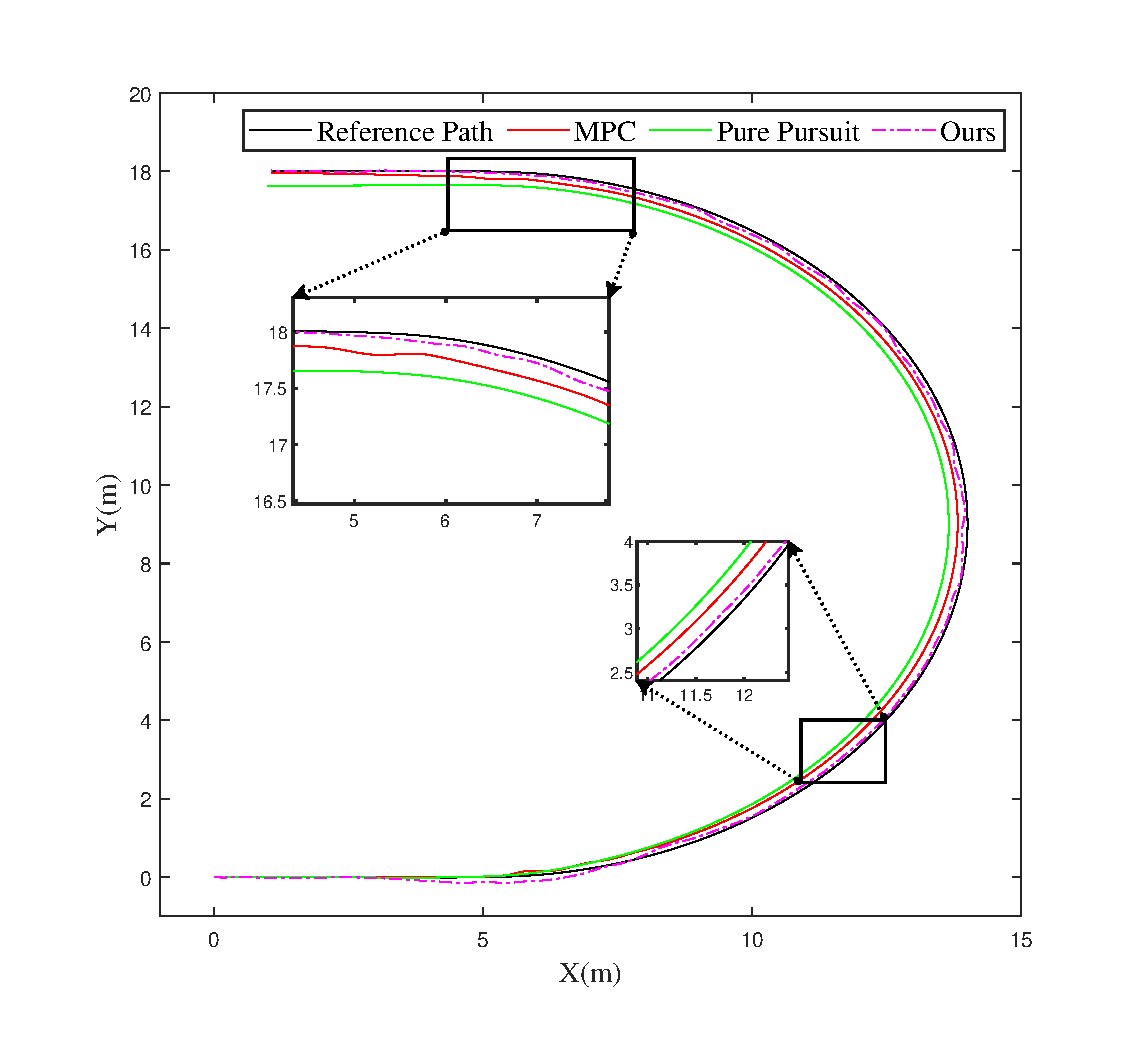
\includegraphics[width=0.9\linewidth]{track1}
	\caption{Effect of preset trajectory tracking}
	\label{fig:Effect}
\end{figure}


Figure \ref{fig:Effect} shows the qualitative effects of the three trajectory tracking. For quantitative analysis, we compare the performance metrics of 3 methods regarding the lateral error, heading error, response time, and trajectory tracking time. As shown in the table \ref{tab:per_traj_1}, the response time of the proposed algorithm is similar to that of the pure pursuit algorithm and much smaller than that of the MPC algorithm.

Regarding trajectory tracking time, it can be seen from figure.\ref{fig:Effect} that the proposed algorithm travels a path length greater than the two algorithms, which is basically equal.


\begin{table}[h]
	\begin{center}
		\caption{Performance analysis in preset trajectory tracking}
		\label{tab:per_traj_1}
		\begin{tabular}{ccccccc}
			\toprule
			\multirow{2}*{Method} & Lateral error(m) & Heading error(deg) & \multicolumn{3}{@{}c@{}}{Response time(ms)} & Travel time(s) \\
			\cmidrule{4-6}
			&Mean & Mean & Min & Max & Mean & Mean \\
			\midrule
			Ours           & \textbf{0.07}  & 5.08         & 2.33 & 6.63         & 2.84  & 39.45 \\
			Pure pursuit & 0.28   & \textbf{4.37}     &0.04  & 0.05     & 0.15 & 36.14\\ 
			MPC         & 0.15  & 4.65   &32.50 & 120.01         & 43.97  & 36.31  \\
			\botrule
		\end{tabular}
	\end{center}
\end{table}

As shown in Figure \ref{Fig:Head_error1},our method has similar mean values as the other methods in terms of heading error. However, it has a smaller error distribution, which indicates that our method is more stable in the control of the heading. For the lateral error shown in Fig.~\ref{Fig:Lateral_error1}, the average value of the lateral error and the  distribution of lateral error in the range of $25\%-75\%$ of the proposed method are smaller than those of MPC and pure pursuit methods, with small fluctuations and stable lateral error. This indicates that our method has apparent advantages in tracking control of the lateral error.
Therefore, our designed controller is still inadequate in heading error control. However, our method is more stable, and the relatively more important lateral error control effect is better than the other two controllers.
\begin{figure}[!htbp]
	\centering
	\subfloat[]{\label{Fig:Lateral_error1}%
		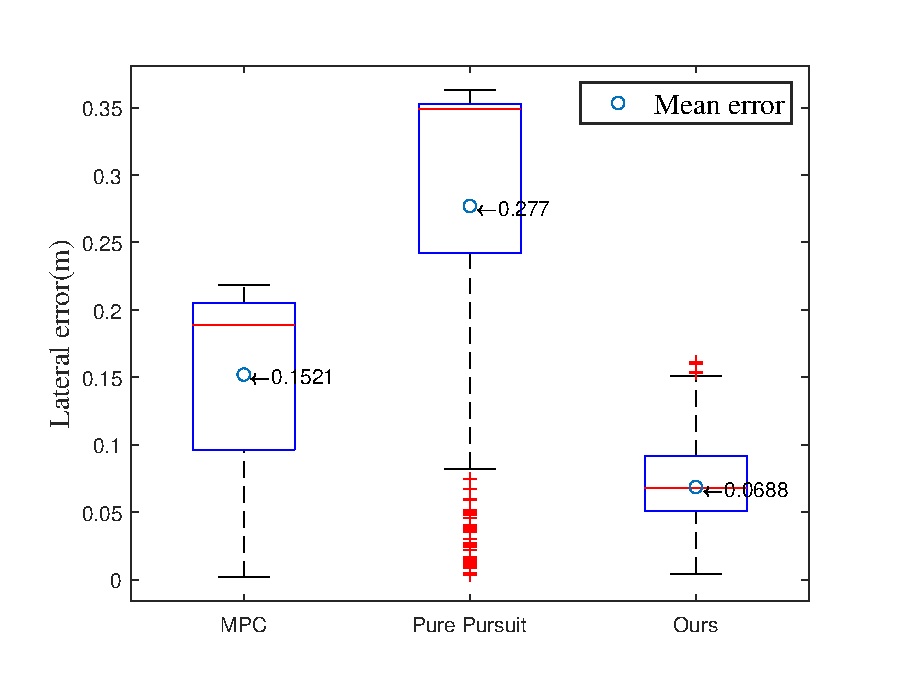
\includegraphics[width=0.45\textwidth]{Later1}}
	\quad
	\subfloat[]{\label{Fig:Head_error1}%
		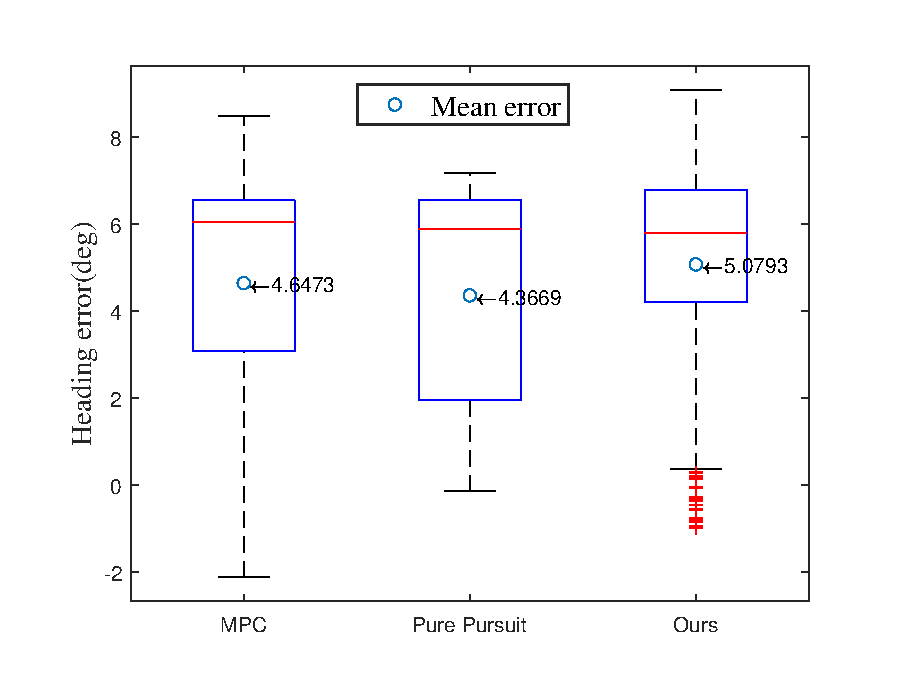
\includegraphics[width=0.45\textwidth]{head1}}  
	
	\caption{Evaluation of preset trajectory tracking in the simulator \protect\subref{Fig:Lateral_error1} Statistics for lateral errors,\protect\subref{Fig:Head_error1}Statistics for heading errors}
	\label{Fig:Statistics1}
\end{figure}

\subsubsection{Planning trajectory tracking}
In the task of planning trajectory tracking, as illustrated in Figure. \ref{fig:actual_trajectory}, we created a simulation environment in Gazebo to model the lane change scenario for unmanned vehicles. The reference trajectory is generated by the front-end planner, and then we evaluate the tracking performance of three trajectory tracking algorithms as shown in Figure.\ref{fig:traking2}. The lateral error and heading error statistics during the tracking process are shown in Figure.\ref{Fig:Statistics2} and \ref{Fig:Statistics3}. As observed in the figure, the average value of the heading error of the proposed method is similar to the other two methods. However, the lateral distance statistics closely follow the desired path, indicating minimal changes in lateral error and more stable lateral tracking.
\begin{figure}
	\centering
	\includegraphics[width=0.9\linewidth]{actual_trajectory}
	\caption{Planning environment}
	\label{fig:actual_trajectory}
\end{figure}

\begin{figure}
	\centering
	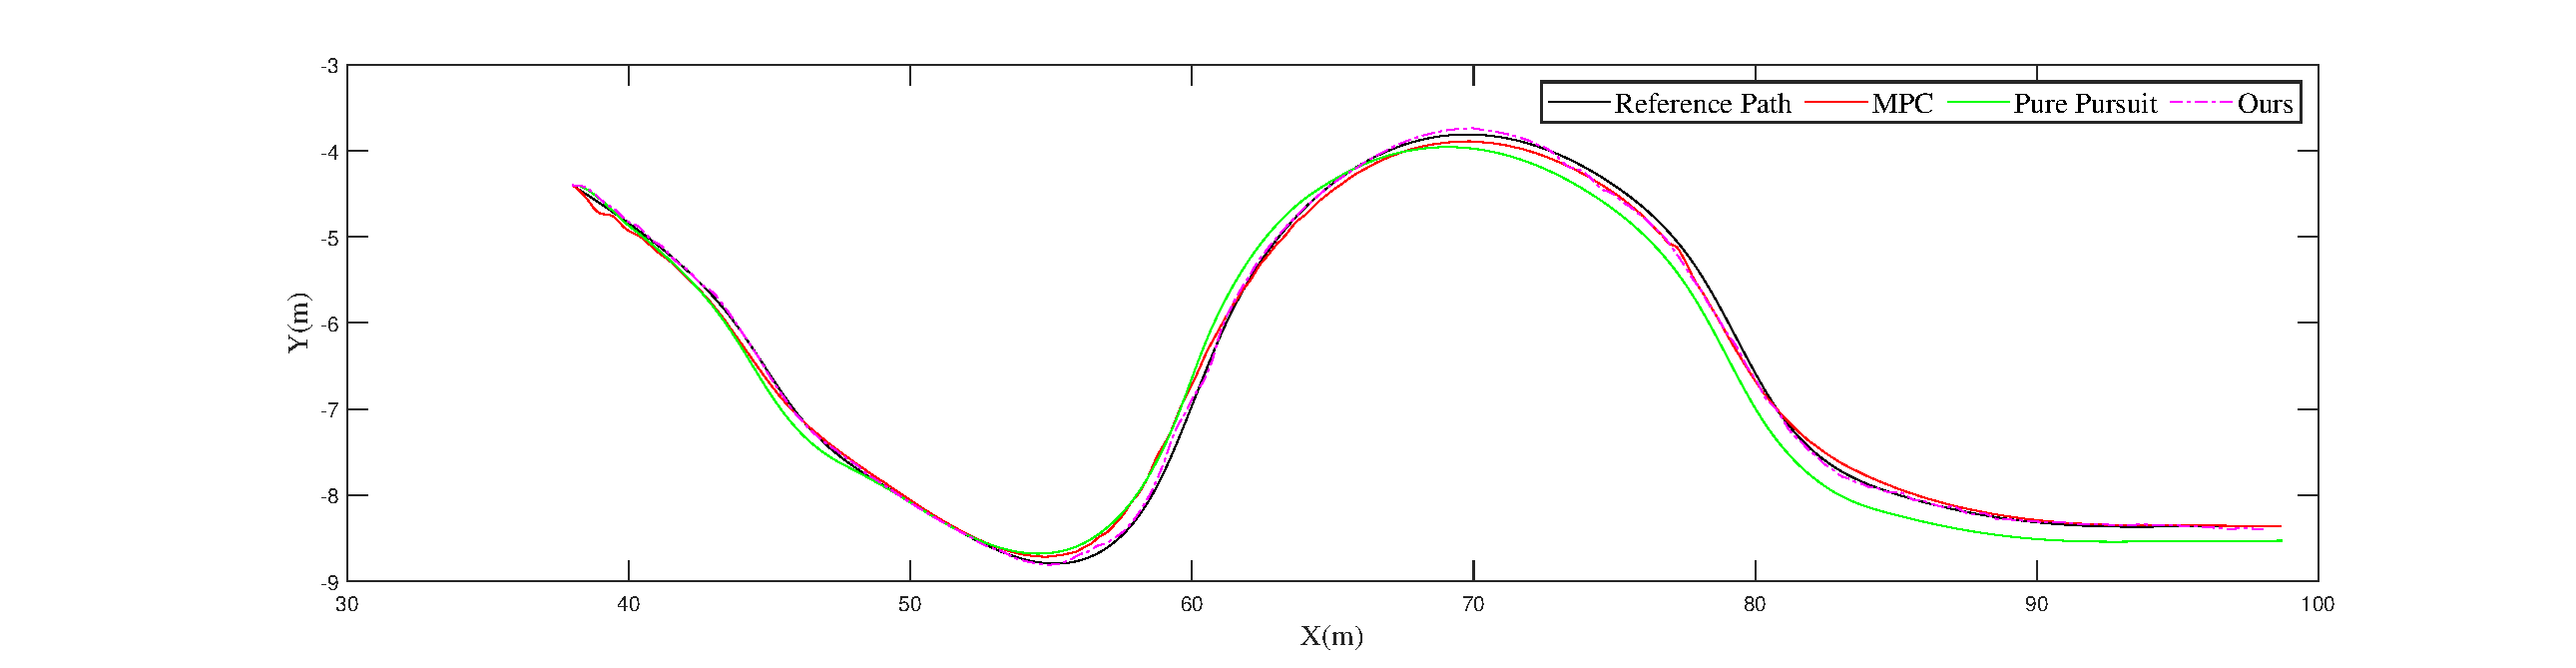
\includegraphics[width=1.0\linewidth]{track2}
	\caption{Effect of planning trajectory tracking}
	\label{fig:traking2}
\end{figure}



\begin{figure}[!htbp]
	\centering
	\subfloat[]{\label{Fig:Lateral_errors2}%
		\includegraphics[width=0.45\textwidth]{Laterals2}}
	\quad
	\subfloat[]{\label{Fig:Lateral_error2}%
		\includegraphics[width=0.45\textwidth]{Lateral2}}  
	
	\caption{Statistics for lateral errors. \protect\subref{Fig:Lateral_errors2}  Variation of lateral error with arc length,\protect\subref{Fig:Lateral_error2}Box plot of lateral error }  
	\label{Fig:Statistics2}
\end{figure}

\begin{figure}[!htbp]
	\centering
	\subfloat[]{\label{Fig:Head_errors2}%
		\includegraphics[width=0.45\textwidth]{heads2}}
	\quad
	\subfloat[]{\label{Fig:Head_error2}%
		\includegraphics[width=0.45\textwidth]{head2}}  
	
	\caption{Statistics for heading errors \protect\subref{Fig:Head_errors2} Variation of heading error with arc length,\protect\subref{Fig:Head_error2}Box plot of heading error}
	\label{Fig:Statistics3}
\end{figure}


Table \ref{time} presents the results of our performance comparison among different trajectory tracking approaches in terms of time. Notably, the Pure Pursuit method exhibits a shorter completion time and response time compared to the other two methods, owing to its mechanism of minimizing the lateral error via adjusting the front wheel rotation angle during tracking. However, this approach suffers from poor performance in terms of lateral errors. On the other hand, the completion time of the MPC method is similar to our proposed approach. However, its response time is considerably higher than the other two methods, with a maximum response time of up to 150.76 ms. Conversely, our proposed method exhibits a response time compared to the Pure Pursuit method but achieves superior tracking performance in lateral error. These findings indicate that our method is capable of providing rapid and accurate trajectory tracking performance in complex scenarios.
\begin{table}[h]

	\begin{center}

		\begin{minipage}{\textwidth}

			\caption{Evalution time in the simulator}\label{time}

			\begin{tabular*}{\textwidth}{@{\extracolsep{\fill}}lcccc@{\extracolsep{\fill}}}

				\toprule%
				\multirow{3}*{Method} 	
				& \multicolumn{3}{@{}c@{}}{Response Time(ms)} & \multicolumn{1}{@{}c@{}}{Travel Time(s)} \\\cmidrule{2-4}%\cmidrule{5-5}

				        & Max & Mean & Min &  Mean \\

				\midrule

				Ours   & 4.67  & 2.76 & 2.37 & 69.49 \\

				MPC  & 150.76  & 41.14  &33.64  & 69.40  \\

				Pure pursuit & 0.17&0.06 & 0.03 &63.10 \\ 
				\botrule

			\end{tabular*}

			\footnotetext{}


		\end{minipage}

	\end{center}

\end{table}

\section{Conclusion}\label{sec4}
In this paper, a trajectory tracking controller based on the Dueling DDQN reinforcement learning method is proposed. This approach involves separating the state information encoding network from the unmanned vehicle policy network and introducing a self-attention mechanism to achieve effective feature extraction and encoding of state information. To train our approach, we establish an interactive environment using the Gazebo simulation and design a multi-task intensive reward function for trajectory tracking.

The comparison experiments show that the reinforcement learning trajectory tracking controller proposed in this paper has an excellent performance in terms of response time and lateral error compared with the traditional pure pursuit trajectory tracking method and MPC based method. However, it does not improve much in heading error and is not suitable for scenarios with high requirements for heading error. In future research, discrete acceleration can be considered as the input to increase the controllable range of vehicle speed and enhance heading tracking performance.

\bmhead{Acknowledgments}

This work was supported by Natural Science Foundation of Hebei Province (F2022203040, F2020203016), Natural Science Foundation of China (62073277, 62188101), Central Government Guided Local Science and Technology Development Fund Project (226Z0301G), Key R \& D Program of Hebei Province (20311803D), Hebei Innovation Capability Improvement Plan Project (22567619H).




\section*{Declarations}
\begin{itemize}
	\item \textbf{Conflict of interest/Competing interests} Not applicable
	\item \textbf{Ethics approval} Not applicable
	\item \textbf{Consent to participate} Not applicable
	\item \textbf{Consent for publication} Not applicable
	\item \textbf{Availability of data and materials} Not available
	\item \textbf{Code} Not available
	\item \textbf{Authors'contributions}:  
 	\textbf{Weiming Liao:} Methodology, Software, Writing-Original draft preparation. \textbf{Guanglei Zhou:} Research ideas, Writing-Reviewing. \textbf{Zihao Chen:} Data curation,Investigation.
\end{itemize}







%%===========================================================================================%%
%% If you are submitting to one of the Nature Portfolio journals, using the eJP submission   %%
%% system, please include the references within the manuscript file itself. You may do this  %%
%% by copying the reference list from your .bbl file, paste it into the main manuscript .tex %%
%% file, and delete the associated \verb+\bibliography+ commands.                            %%
%%===========================================================================================%%

\bibliography{rl-tracking}% common bib file
%% if required, the content of .bbl file can be included here once bbl is generated
%%\input sn-article.bbl

%% Default %%
%%\input sn-sample-bib.tex%

\end{document}
